\section{Introduction} \label{introduction}

Murder mysteries as a genre first became popular in the 19th century in literature.
They then quickly grew in popularity over the next decades.
These detective stories reached their height of popularity in the 1920s and 30s, which has since been referred to as the Golden Age of Detective fiction.
Many authors from that time are still prevalent in today's pop culture, as can be seen by for example the 2017 movie adaptation of Agatha Christie's novel \emph{Murder on the Orient Express}.
Novels from that era often follow very strict rules as defined for example by Van Dine's \emph{Twenty Rules for Writing Detective Stories} \cite{van_dine_1928} or Knox' \emph{Ten Commandments} \cite{knox_1929}.

Today, murder mysteries have found their way into most genres.
Television series and movies feature them especially often.
These crime shows come in a huge variation of sub-genres, be it the classical detective story or a more outlandish setting, whether it is a Zombie helping to solve crime by eating the victims brains\footnote{\url{https://www.imdb.com/title/tt3501584/?ref_=nv_sr_1}} or the devil himself coming to earth to find who did it\footnote{\url{https://www.imdb.com/title/tt4052886/?ref_=fn_al_tt_1}}.
The board game \emph{Cluedo} is another representation of this genre, letting the players compete on who can solve the murder of Dr. Black the fastest\footnote{\url{https://shop.hasbro.com/en-us/product/clue-game-2013-edition:9BCB9C5E-5056-9047-F505-6D1166C5961E}}.

\subsection{Procedural Murder Mystery Generation}

\begin{figure}
  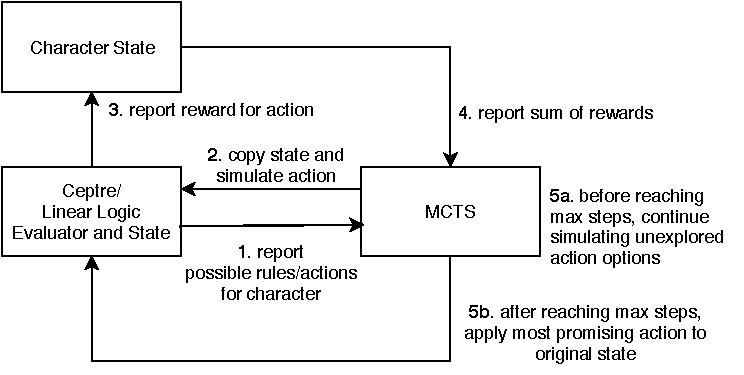
\includegraphics{mcts-flow.pdf}
  \caption{The communication between the three core elements of our system. When tasked with deciding on an character's next move, the MCTS component continuously creates copies of the simulation state to explore which sequence of actions provides the given character with the highest reward, until a maximum number of steps has been taken.}
  \label{fig:mcts-components}
\end{figure}


Murder mysteries in video games often follow a linear, pre-written path that may include branching options.
The extent to which games divert from this mode of storytelling will be explored in Section \ref{related_work}.
Rather than replacing authors by generating stories automatically, this project aims to provide a tool for authors to craft rules that inform the mechanics of a world.
These mechanics, combined with a procedural simulation, then yield a generated narrative whose quality will largely depend on the complexity of the pre-authored rules.
Using this system instead of a branching narrative promises a higher degree of variability and the possibility of emergent, perceived creativity in the stories on each playthrough.
The characters in the simulation use the low-level rules to act in ways that the player recognizes as intelligent, planning behavior.
The stories generated in this way lend themselves better to be displayed in an amusing puzzle setting, rather than a highly dramatic story that is authored to provide the best pacing and suspense.

Our system uses Ceptre \cite{martens_2015} as a basis. Ceptre is a system to formulate and run interactive narratives or simulations.
We extend Ceptre's core concept with non-deterministic outcomes and a reward system for actions to drive artificial agents.
Our simulation is neither driven by a human player or random choices, which are the two options Ceptre offers.
Instead, we implement MCTS agents that drive the story by evaluating the possible options to maximize their reward.
An illustration of the communication between Ceptre, the MCTS system, and the agents can be found in figure \ref{fig:mcts-components}.
To make predicting the outcome of the simulation multiple steps ahead feasible in terms of performance, we re-implemented Ceptre's engine in Python.

In Section \ref{related_work} we will introduce related work in the fields of murder mysteries in video games, procedural story generation, and the story generation system Ceptre.
Section \ref{approach} will explain our approach to our own linear logic evaluator, our rule set, believable agent system, and the game's user interface.
The Section \ref{evaluation} discusses, in particular, our opinion on linear logic in this system and the challenges coming with the authorship of the rules.
Sections \ref{future_work} and \ref{conclusion} will talk about possible next steps that would drive this project further and provide a summary of our findings.
